\section{Bias-variance framework}

The bias-variance framework provides a structured approach for evaluating model performance.
\begin{definition}[\textit{Data}]
    Data are described as:
    \[t_i=f(\textbf{x}_i)+\varepsilon\]
    where $\mathbb{E}\left[\varepsilon\right]=0$ and $\text{Var}\left[\varepsilon\right]=\sigma^2$. 
\end{definition}
\begin{definition}[\textit{Model}]
    The model is represented as:
    \[\hat{t}_i=y(\textbf{x}_i)+\varepsilon\]
    learned from a sampled dataset $\mathcal{D}=\left\{ \textbf{x}_i,t_i \right\}$. 
\end{definition}
\begin{definition}[\textit{Performance}]
    Performance is quantified by:
    \[\mathbb{E}\left[ {\left( t-y(\textbf{x}) \right)}^2 \right]\]
    which measures the expected squared error.
\end{definition}
Hence, the expected squared error can be decomposed as follows:
\begin{align*}
    \mathbb{E}\left[ {\left( t-y(\textbf{x}) \right)}^2 \right]   &= \mathbb{E}\left[ \left( t^2+y{(\textbf{x})}^2-2ty(\textbf{x}) \right) \right] \\
                                                                &= \mathbb{E}\left[ t^2  \right]+ \mathbb{E}\left[y{(\textbf{x})}^2 \right]- \mathbb{E}\left[2ty(\textbf{x}) \right] \\
                                                                &= \mathbb{E}\left[ t^2  \right] + \mathbb{E}{\left[ t \right]}^2 - \mathbb{E}{\left[ t \right]}^2+ \mathbb{E}\left[y{(\textbf{x})}^2 \right] +  \mathbb{E}{\left[y(\textbf{x}) \right]}^2 - \mathbb{E}{\left[y(\textbf{x}) \right]}^2 -  2f(\textbf{x})\mathbb{E}\left[y(\textbf{x}) \right] \\
                                                                &= \text{Var}\left[ t  \right] + \mathbb{E}{\left[ t \right]}^2+ \text{Var}\left[y(\textbf{x}) \right] +  \mathbb{E}{\left[y(\textbf{x}) \right]}^2 -  2f(\textbf{x})\mathbb{E}\left[y(\textbf{x}) \right] \\
                                                                &= \text{Var}\left[ t  \right] +  \text{Var}\left[y(\textbf{x}) \right] +  {\left(f(\textbf{x}) -\mathbb{E}\left[y(\textbf{x}) \right]\right)}^2 \\
                                                                &= \underbrace{\text{Var}\left[ t  \right]}_{\sigma^2}  +  \underbrace{\text{Var}\left[y(\textbf{x}) \right]}_{\text{variance}}  +  \underbrace{\mathbb{E}{\left[f(\textbf{x}) -y(\textbf{x}) \right]}^2}_{\text{squared bias}} 
\end{align*}
\begin{figure}[H]
    \centering
    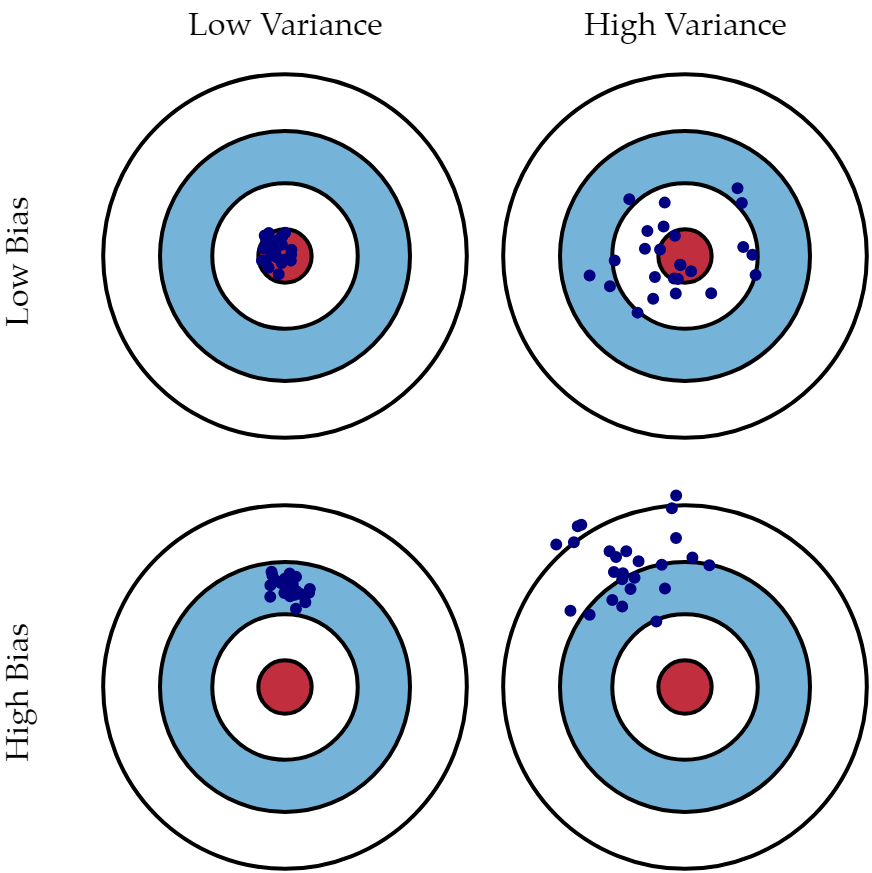
\includegraphics[width=0.5\linewidth]{images/bvf.png}
    \caption{Bias-variance framework}
\end{figure}

\paragraph*{Model variance}
When we sample multiple datasets $\mathcal{D}$, we obtain distinct models $y(\textbf{x})$. 
Variance quantifies the dissimilarity between each model learned from a specific dataset and our anticipated learning outcome:
\[\text{variance}=\int \mathbb{E}\left[ {\left( y(\textbf{x}-\bar{y}(\textbf{x})) \right)}^2 \right]\text{P}(\textbf{x})d\textbf{x}\]
The variance diminishes by simplifying the model or increasing the sample size.

\paragraph*{Model bias}
Bias gauges the disparity between the truth ($f$) and our expected learning outcome ($\mathbb{E}\left[y(\textbf{x})\right]$):
\[\text{bias}^2=\int {\left(f(\textbf{x})-\bar{y}(\textbf{x})\right)}^2 \text{P}(\textbf{x})d\textbf{x}\]
Bias decreases with more complex models.
\begin{definition}[\textit{Data noise}]
    Data noise ($\sigma^2$) represents the variance of data and remains constant regardless of data sampling or model complexity.
\end{definition}

\begin{figure}[H]
    \centering
    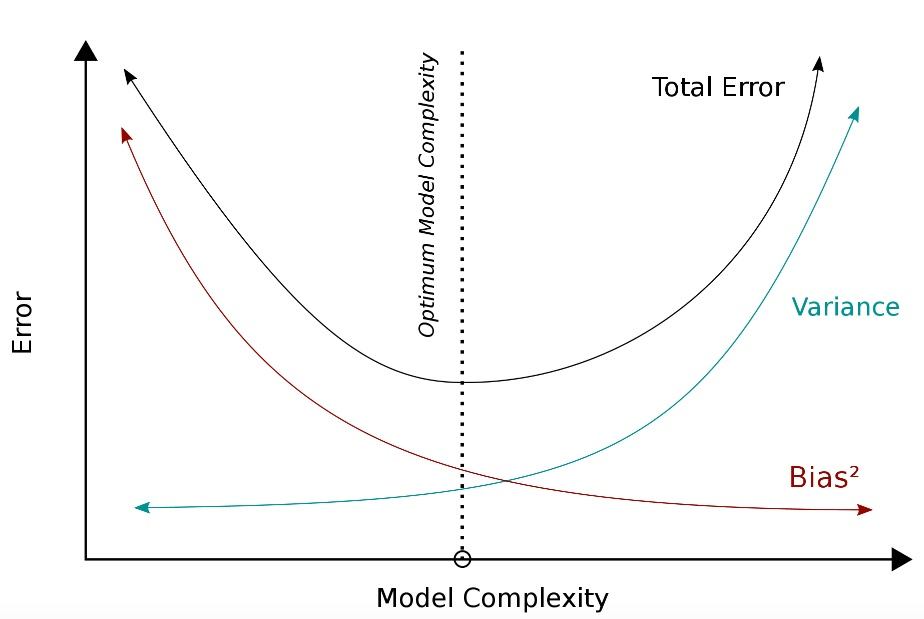
\includegraphics[width=0.5\linewidth]{images/bvf1.png}
    \caption{Bias-variance framework impact}
\end{figure}
In practical terms, the estimation is affected as follows:
\begin{itemize}
    \item High variance leads to overfitting.
    \item High bias results in underfitting.
    \item Low bias and low variance yield a well-balanced approximation.
\end{itemize}
\begin{figure}[H]
    \centering
    \begin{subfigure}{0.32\textwidth}
        \centering
        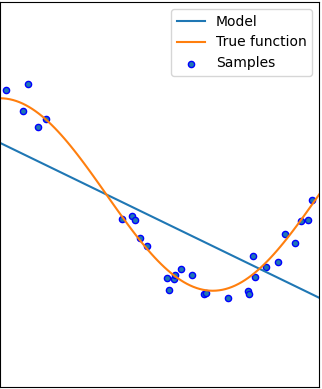
\includegraphics[width=0.75\linewidth]{images/hb.png} 
        \caption{High bias}
    \end{subfigure}
    \begin{subfigure}{0.32\textwidth}
        \centering
        
\includegraphics[width=0.75\linewidth]{images/b.png} 
        \caption{Balanced}
    \end{subfigure}
    \begin{subfigure}{0.32\textwidth}
        \centering
        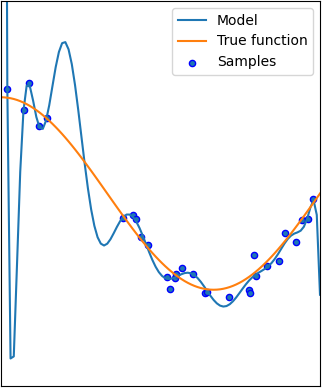
\includegraphics[width=0.75\linewidth]{images/hv.png} 
        \caption{High variance}
    \end{subfigure}
    \caption{Bias-variance balancing}
\end{figure}

\subsection{Regularization and bias-variance}
The bias-variance decomposition elucidates why regularization enhances error reduction on unseen data. 
Lasso surpasses ridge regression when only a few features are linked to the output.